\documentclass{standalone}
\usepackage{tikz}

\usetikzlibrary{shapes,arrows, backgrounds, positioning}
\begin{document}
% \usetikzlibrary{shapes,arrows, backgrounds}

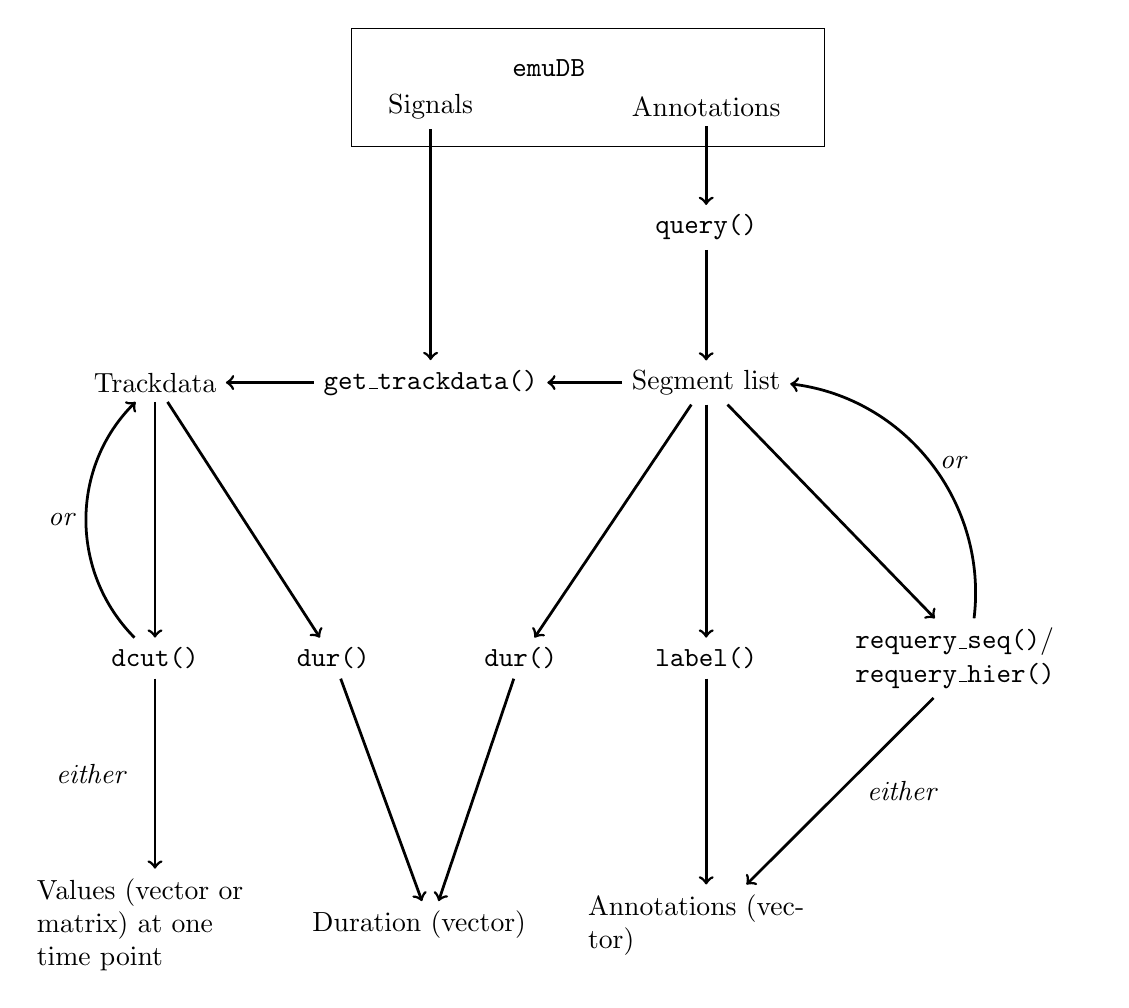
\begin{tikzpicture}[node distance=3.5cm]
  % origin
  \node (origin) {\texttt{get\_trackdata()}};

  %%%%%%%%%%%%%%%%%%
  \draw[] (-1, 4.5) rectangle (5, 3);
  \node () at (1.5, 4) [] {\texttt{emuDB}};

  \node (signals) [above of=origin] {Signals};

  \node (annotationsDB) [right of=signals] {Annotations};

  %%%%%%%%%%%%%%%%%
  \node (query) [below=1cm of annotationsDB] {\texttt{query()}};

  %%%%%%%%%%%%%%%%%
  
  \node (seglist) [right of=origin] {Segment list};

  \node (trackdata) [left of=origin] {Trackdata};

  %%%%%%%%%%%%%%%%%
  \node (dcut) [below of=trackdata] {\texttt{dcut()}};

  \node (dur1) [right=1cm of dcut] {\texttt{dur()}};

  \node (label) [below of=seglist] {\texttt{label()}};

  \node (dur2) [left=1cm of label] [] {\texttt{dur()}};

  \node (requery) [right=1cm of label, text width=3cm] {\texttt{requery\_seq()}/ \texttt{requery\_hier()}};

  %%%%%%%%%%%%%%%%%
  \node (duration) [below=6.3cm of origin, text width=3cm] {Duration (vector)};

  \node (values) [left of=duration, text width=3cm] {Values (vector or matrix) at one time point};

  \node (annots) [right of=duration, text width=3cm] {Annotations (vector)};


  %%%%%%%%%%%%%%%%%%%%
  %%%%%%%%%%%%%%%%%%%%
  \draw [->, line width=1] (signals) to (origin);
  \draw [->, line width=1] (origin) to (trackdata);
  \draw [->, line width=1] (seglist) to (origin);

  
  \draw [->, line width=1] (annotationsDB) to (query);
  \draw [->, line width=1] (query) to (seglist);
  
  \draw [->, line width=1] (trackdata) to (dcut);
  \draw [->, line width=1] (trackdata) to (dur1);
  
  \draw [->, line width=1] (seglist) to (dur2);
  \draw [->, line width=1] (seglist) to (label);
  \draw [->, line width=1] (seglist) to (requery);
  
  \draw [->, line width=1] (dcut) -- node[xshift=-0.8cm]{\textit{either}} (values);
  \draw [->, line width=1] (dur1) to (duration);
  \draw [->, line width=1] (dur2) to (duration);
  \draw [->, line width=1] (label) to (annots);
  \draw [->, line width=1] (requery) -- node[xshift=0.8cm]{\textit{either}} (annots);
  
  \draw [->, line width=1] (dcut) to [bend left=45] node[xshift=-0.3cm]{\textit{or}} (trackdata);
  \draw [->, line width=1] (requery) to [bend right=45] node[xshift=0.3cm]{\textit{or}} (seglist);
  
\end{tikzpicture}

\end{document}
